\begin{figure}[htbp]
\centering
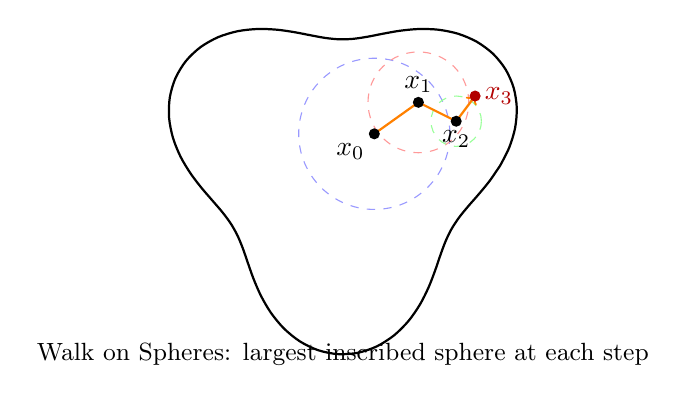
\begin{tikzpicture}[scale=0.8]
  \draw[thick] plot[smooth,domain=0:360,samples=60] (\x:{2.5+0.5*sin(3*\x)}) -- cycle;
  \coordinate (x0) at (0.5,0.5);
  \coordinate (x1) at (1.2,1.0);
  \coordinate (x2) at (1.8,0.7);
  \coordinate (x3) at (2.1,1.1);
  \draw[blue!40,dashed] (x0) circle (1.2);
  \draw[red!40,dashed] (x1) circle (0.8);
  \draw[green!40,dashed] (x2) circle (0.4);
  \draw[->,thick,orange] (x0)--(x1)--(x2)--(x3);
  \fill (x0) circle (2.5pt) node[below left] {$x_0$};
  \fill (x1) circle (2.5pt) node[above] {$x_1$};
  \fill (x2) circle (2.5pt) node[below] {$x_2$};
  \fill[red!70!black] (x3) circle (2.5pt) node[right] {$x_3$};
  \node[font=\small] at (0,-3) {Walk on Spheres: largest inscribed sphere at each step};
\end{tikzpicture}
\caption{Walk on Spheres: from each interior point, jump to a random point on the largest inscribed sphere.}
\label{fig:walk_spheres}
\end{figure}
